\begin{table*}
\begin{minipage}{0.6\linewidth}
    \centering
    \captionof{table}{Ablation Study on \model. All components of \model{} are positively contributing to its performance. }
    \label{tab:ablation}
    \resizebox{0.78\linewidth}{!}{
    \begin{tabular}{l c c}
    \toprule
    \multirow{2}{*}{Model}     & Language Modeling & Reasoning \\
    & ppl $\downarrow$ & acc $\uparrow$ \\
    \midrule
    \midrule
    \rowcolor{mygray} \model{}         &   12.24  &  58.1  \\ 
    \midrule
    w/o DGD                &    13.41     &      56.5     \\
    w/o Momentum           &   13.58  &  56.9  \\
    w/o weight decay            &  13.71   &   57.2  \\
    w/o CMS                     &    13.04      &     57.3     \\
    w/o inner-projection $\vk$  &   13.77  &   56.9  \\
    w/o inner-projection $\vv$  &   13.90  &  55.1   \\
    w/o inner-projection $\vq$  &   12.19  &  57.4   \\
    \toprule
    \end{tabular}
    }
\end{minipage}
~\hfill~
\begin{minipage}{0.37\linewidth}
        \centering
        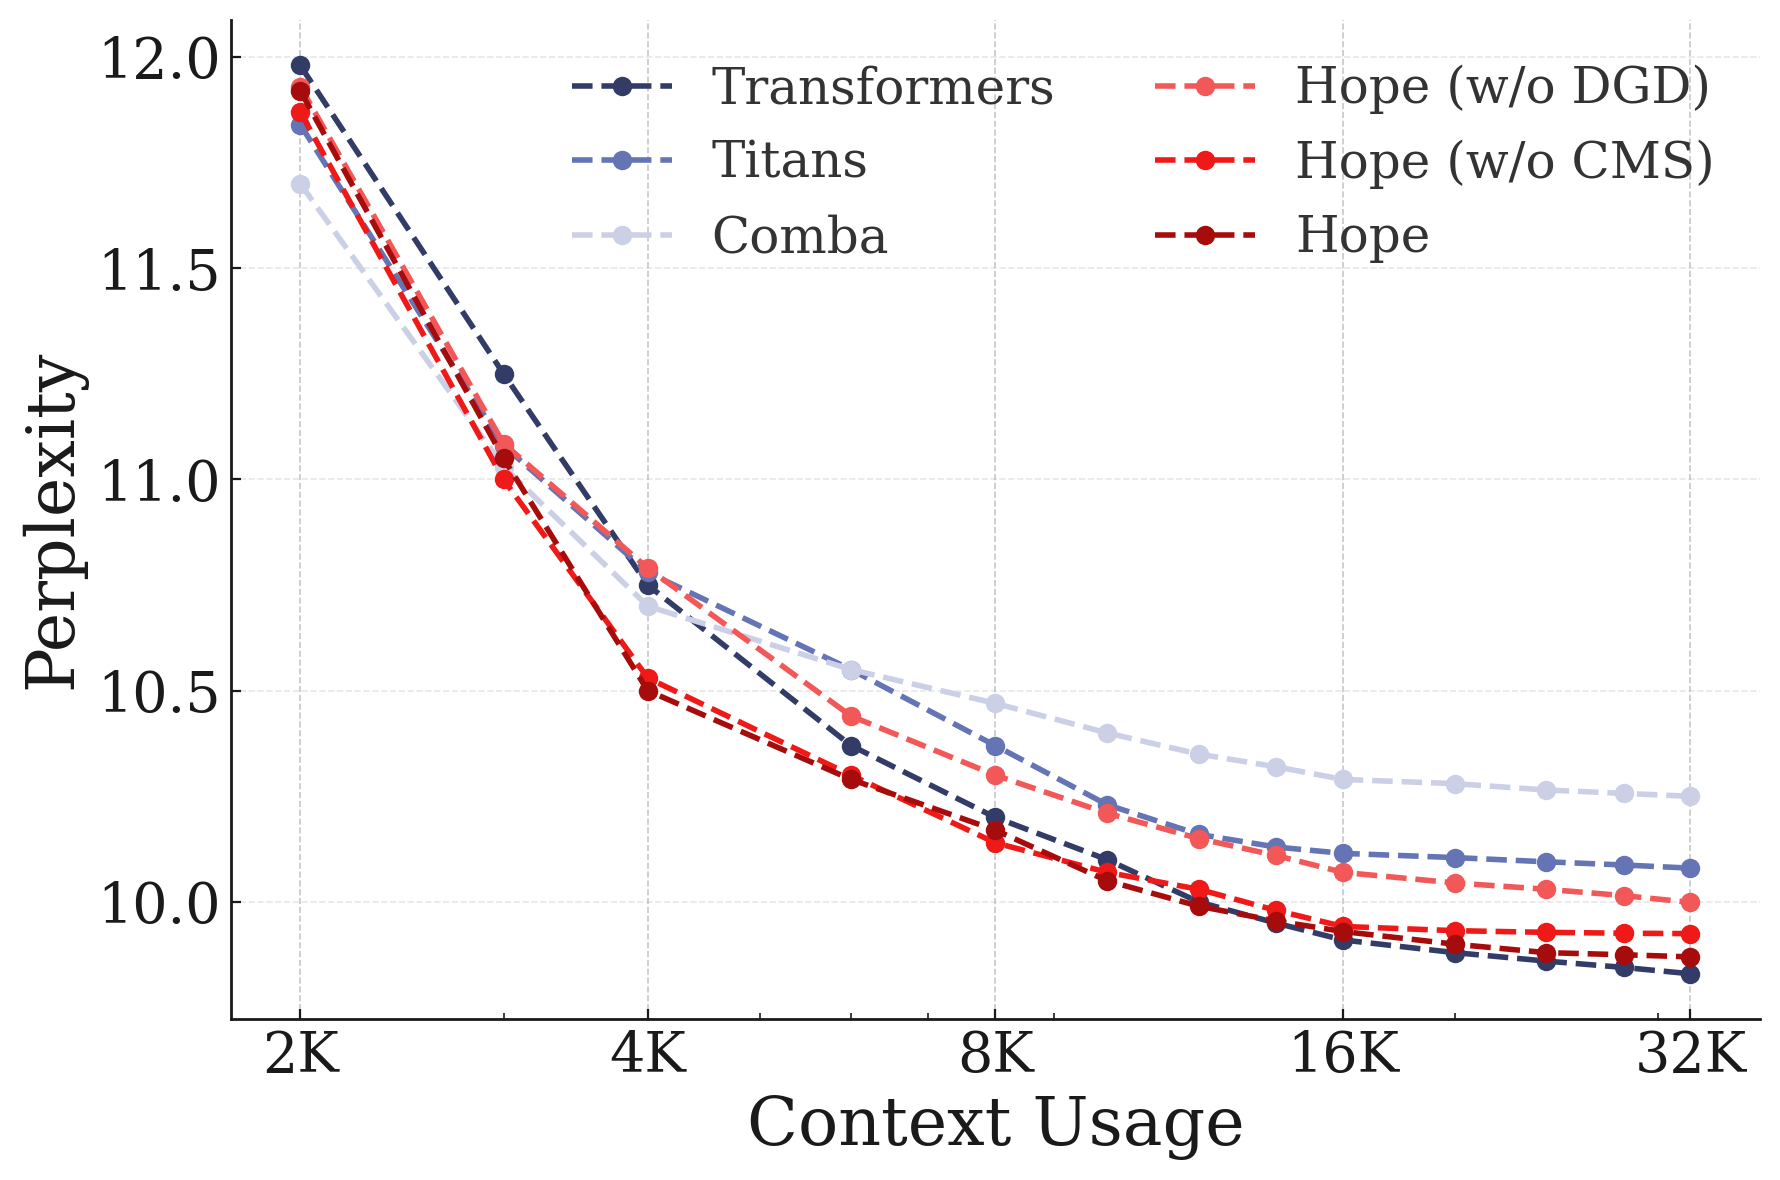
\includegraphics[width=0.87\linewidth]{Images/ablation-context-length.png}
        \captionof{figure}{The effect of context usage on the perplexity of the model. We expect the perplexity of a model with powerful memory management to decrease with more context.}
        \label{fig:placeholder}
\end{minipage}
\end{table*}